%!TEX root=../../thesis_ESG.tex
\chapter{Business context}
\label{chap:business-context}


A Supply Chain is a system of organizations, people, activities, information, and resources involved in producing, transforming or moving a product or service from supplier to customer.
It can be considered for a subsidiary, a whole company or for multiple companies working together.
Its activities extends from the recovery of raw material to their transformation into finished product and their delivery to the costumer.

Supply Chain can fulfill several functions.
Most common are procurement, production, distribution, storage, shipping, sales and billing, and customer relationship.
Works of this thesis deal with optimization of production and storage within companies.


\section{Supply Chain objectives}



Supply Chain management consists in finding the right balance between conflicting objectives.
%Customer satisfaction is based on a trade-off between low cost, appropriate and quality product or service and short delivery lead time.
%To achieve this balance, \ie be competitive, companies and their Supply Chain must face many conflicting objectives.
%Because resources are finite and because of the wide variety of its activities, Supply Chain faces many objectives sometimes contradictory. 
They can be classified into three categories: \emph{costs}, \emph{stocks} and \emph{service}.


Costs are burdens\vl{?} paid by companies as part of their activities.
It can be fixed or variable and direct or indirect.
Fixed costs does not depend on the volume of the business activity like rent, insurance and investment costs (as buying machines).
Opposite\vl{On the other hand}, variable costs, like shipping or energy costs, directly increase with the volume of the business activity.
Direct costs are linked to\vl{concerns} resources entirely dedicated to the product manufacturing like procurement of raw material or worker salaries.
Indirect costs are linked to support functions which are not directly involved in production like marketing, administration.
Commonality of costs is the ability to measure it using a common currency.

\vlil{Je suggère de démarrer par les coûts induits par un stock (inventaire, place, etc) puis de dire que néanmoins le principal cout c'est la ``locked-in money'' qui remplace des investissement pour se développer etc. Ce qui permet de justifier le côté ``à part''}
Stocks, also called \emph{inventory}, are not \vl{really} a cost.
They are similar to working capital.
It is locked-in money until they are transformed (for raw material) or sold (for finished products).
Moreover, storage of stocks \vl{induce costs for storage space, insurance, broken or stolen goods, work time to keep registered stock accurate...} requires space an time to check that real stock correspond to registered stock (part of stock could have been broken, depreciated, or stolen).
Thus, because of their specificity, they must form their own category in optimization process.

\vlil{stock out and replenishment cycle not defined : lexique ?  footnote ?}
Service or \emph{service level} measures the ability of Supply Chain to deliver the right product to customer respecting the deadlines.
There are many indicators to measure service level but we can identify two main categories: \emph{cycle service level} and \emph{fill rate service level}.
Cycle service level is the expected\vl{?} probability of not hitting a stock-out during the next replenishment cycle, and thus, it is also the probability of not losing sales.
Fill rate service level represents the fraction of demand that is delivered without delays or lost sales.
The choice of the indicator depends on the industry.
Indeed, in case of complex products like in aeronautics, if one item is missing in the command, it can delay the whole project.
Thus delivering the whole command is more important. \vl{leading to selecting cycle service lvel}
In case of simple products like in mass distribution, it is more relevant to measure the part of demand delivered at due date. \vl{hence selecting fill rate service level.}


\medskip


Automotive and luxury industries are good example of these conflicting objectives.
In automotive industry, high stock is impossible because of depreciation and diversity of products.
However, service level must be high due to high competition.
In luxury industry, availability of the right product in the right store is more critical than production cost but high stock are still impossible.


In general, \emph{industrial agility} which is the ability to face variations in customers' demand is an efficient way to be competitive if two conditions are satisfied.
First, cost of agility must\vl{should stay} be reasonable and second, agility must\vl{should} not be achieve thanks to high stocks.
For a company, defining its agility is therefore exactly finding a balance between cost, stock and service.


Industrial agility can be split in two parts: \emph{capacitative reactivity} and \emph{flexibility}.
Capacitative reactivity is the ability to face variations on the global volume.
\vlil{for example by being able to produce more product than the estimated demand (industrial overcapacity)}
A common way to deal with it is an industrial overcapacity.
Capacitative reactivity is more critical in sector like process industry since adding overcapacity is extremely expensive and outsourcing can be extremely hard.
Flexibility is the ability to face variations of the products mix.
Multi-sourcing its production \vl{quick def} enables more flexibility but decreases productivity.
Another way to increase flexibility consists in increasing stocks.
Among other, flexibility enables to adapt to an unexpected cannibalization of a product by another.
Luxury industry and mass distribution are probably the sectors where being flexible is the most critical due to the huge number of products.


Defining its agility depends on the industry but also on the decision level: strategic (long-term), tactic (mid-term) or operational (short-term).
%Definition of long-term, mid-term and short-term horizon are not expressed in term of days but in term of kind of decision.
At the strategic level, the executive committee has expressed the desired agility and wants to decide investment in production capacities.
Thus, agility is a constraint, cost is an objective to minimize and stock is secondary if not considered.
At the frontier of strategic and tactic level, capacitative reactivity cannot be changed, S\&OP process has expressed a desired service level and wants to decide multi-sourcing.
Thus, service level is a constraint and cost is an objective.
At the tactic level, service level is an input for the production planning and stock and production are the lever.
Thus, service level is a constraint, stock is an objective to minimize and production are the decisions.
At the operational level, last-minute trade-offs are made like scheduling.



% \begin{itemize}
%   \item \emph{Costs.} Standard examples are investment costs (purchase of plants, warehouse or machines), production costs (salaries) or shipping costs (regardless of transportation mode, of rental or purchase).

%   \item \emph{Stocks.} Even if it looks like a cost, stocks have their own characteristics.
%   They correspond to working capital and they cannot be compared to industrial costs.
%   - argent immobilise
%   - vol
%   - faire inventaire
%   - dépréciation

%   \item \emph{Service.} It measures the ability of Supply Chain to deliver the right product with respect to deadlines.
% \end{itemize}
% \esgil{Faire un paragraphe ? \emph{Flexibility}, which is the ability to face variations of the products mix, or \emph{capacitative reactivity}, which is the ability to face variations on the global volume, are also costs since it implies investments.}

% \esgil{Faire trois paragraphe plus fourni sur chacune des parties.}

% In an ideal case, cost and stock must be very low whereas service must be very high.
% However, it is easy to see the contradictions.
% In automotive industry, high stock is impossible because of depreciation an diversity of products.
% However, service level must be high which requires a huge flexibility.
% In luxury industry, availability of the right product in the right store is more critical than manufacturing cost.
% Among other examples, over-capacity increases flexibility but is expensive or specialization of assembly lines or plants increases productivity but often reduces flexibility.
% Depending on the industry, a trade-off between these three incomparable objectives must be found.
% The decision-maker must define which one is the objective and which ones are constraints or simply ignored.


\section{Supply Chain organizations}


Supply Chain organizations can be classified into four main models \cite{arnold2007} which are represented in \cref{fig:supply-chain-models}.
\vlil{maybe a second example for each organization}

\begin{itemize}
  \item \emph{Engineer-To-Order (ETO).}
  The customer is involved in the design and gives engineering requirements and specifications which enables much customization and a specific design.
  The consequences are long delivery lead times due to purchasing of raw material and to designing.
  Classical domains are aeronautic or aerospace industries.

  \item \emph{Make-To-Order (MTO).}
  Products are made from standard items but with custom-designed components.
  Therefore, inventory are only composed of raw material and delivery lead time are still long.
  For example, marine energy turbines can be produced with a MTO organization.

  \item \emph{Assemble-To-Order (ATO).}
  Customer involvement is limited to selection of component options.
  Thus, inventory is only composed of semi-finished products ready for assembly items and delivery lead time are short.
  Production of laptops partially follows this organization.

  \item \emph{Make-To-Stock (MTS).}
  Customer has very little involvement in the design.
  Products are engineered and manufactured to fill stocks which supplied clients demand.
  This organization enables the shortest delivery lead time.
  The majority of mass distribution products uses this organization.
\end{itemize}
For some products, best organization is obvious due to size of series.
For example, a French aeronautic company produces engine of an aircraft carrier with a ETO organization  turboshaft of chopper with MTO organization.
For other industries, identifying the best organization also depend on the commercial strategy (laptops may also be produced with MTS organization) and is critical to define which decisions are short-term, mid-term or long-term and to know when costs, stock and service can be impacted.


\begin{figure}[h]
  \centering
%  \includegraphics[width=\textwidth]{main/introduction/images/.tikz}
  \esgil{Include figure of the 5 supply chain models ou celle de la formation APICS (slide 4)}
  \caption{Scheme of Supply Chain organizations}
  \label{fig:supply-chain-models}
\end{figure}



\section{Presentation of Argon Consulting}


Argon Consulting is an international, independent consulting firm whose mission is to help its clients achieve sustainable competitive advantage through operational excellence.
It began its consultancy activity in 2001 and employs over 230 consultants in six offices: Paris, London, Atlanta, Singapore, Melbourne and Mumbai.


Argon consulting has supported many companies in operational transformation projects (R\&D, Procurement, Manufacturing, Supply Chain, Distribution, Services, SG\&A, Performance Management, Change Management).
Industries served cover
\emph{Aerospace \& Defense} (Lat\'eco\`ere, Safran, Thales) and
\emph{Discrete Manufacturing} (Alstom, SNCF, DCNS) which have small-series and large program logic as well as
\emph{Retail} (ADEO, Carrefour, Cdiscount) which sells products or services to large number of customers through multiple channels of distribution.
In the mid of these extremes, we also find
\emph{Automotive} (Michelin, PSA, Valeo) where innovation performance and diversity of products are challenging,
\emph{Consumer Packaged Goods} (Bel, Danone, L'Oréal) where decreasing consumption and fluctuation of productions costs reduce profitability, and
\emph{Textile} (Galeries Lafayette, Cama\"ieu, Kiabi) where fast product renewal and fast evolution of sourcing are critical at operational level.
Among other sectors with specific rules,
\emph{Luxury Goods} has highly erratic demand and is extremely competitive,
\emph{Pharmaceutical Industry} (Merck, Sanofi, Servier) has economic pressure applied by state authorities due to imbalance of the health insurance systems and
\emph{Energy \& Utilities} (EDF, ENGIE) is capital-intensive, highly cyclical, fully globalized and at the heart of geostrategic issues.


Argon Consulting began as a consultancy company specialized in logistic.
Growing, it acquired expertise at every level of Supply Chain.
Argon Consulting describes itself as a multi-specialized firm whose competitive advantage comes from its ability to quantify their studies.
Through this thesis, the objective is to find an unified framework for some recurrent problems.
Moreover, Argon Consulting wants to scientifically test the accuracy and efficiency of the models developed.






\section{Argon Consulting's clients cases}


Argon Consulting's clients cases considered in this thesis fall into Assemble-To-Order and Make-To-Stock organizations.
We study two cases in this thesis.
First case is tactic.
It occurs when flexibility of means of production is already defined and we aims at deciding stock and production \vl{levels} which enable to achieve the desired service level.
Second case is more strategic.
It occurs when capacity reactivity is already defined and we aims at deciding the multi-sourcing of production which will ensure enough flexibility at tactic and operational level.


\subsection{Production planning}
\label{sec:business-context:argon:pdp}


Production planning is part of the production function of the Supply Chain and occurs at tactic level when flexibility of means of production is already defined.
In Assemble-To-Order and Make-To-Stock organizations, stocks are the last levers on flexibility and must be sufficient to serve demand at due date.
Then, production planning problem consists in deciding the orders of production, \ie when production starts and how much is produced, which defines stocks and enables to achieve the desired service level.


Difficulties of this problem come from many factors\vl{constraint} which prevent last minute production.
First, production capacities are limited.
Thus, production must be anticipated in order to deliver peak selling season, promotion program, vacation shutdown, etc.
It leads to inventory called \emph{anticipation inventory}.
Second, demand and lead time have random variations.
If demand or lead time are greater than forecast, a stock-out can occur.
To prevent it, \emph{safety stocks} are kept as a reserve.
Finally, since \emph{flexibility} of means of production is limited, \emph{lot-size inventories} also called \emph{cycle stocks} are needed.
%They form the portion of inventory that decreases gradually as customers demand is satisfied and that are replenished cyclically when suppliers’ orders are received.
They form the portion of stocks that varies over time due to production and demand satisfaction.
\esgil{Ajouter la figure en dent de scie avec les différents stock}


\medskip


Production planning aims at minimizing \vl{cumulated} stocks subject to constraints defined at higher level.


Service level is the first constraint.
In our case, Argon Consulting's clients want to reach a desired service level which depends on the strategy of the company.
It is a trade-off between several objectives as loss of reputation, intended costs, risk, benefits, etc.
Production planning problems take it as an input since service level is a long-term decision whereas production decisions are mid-term decisions.
Since we are interested in Assemble-To-Order and Make-To-Stock models, we will consider mainly fill rate service level. \vl{as defined in}


Industrial costs are another constraint.\vl{unclear}
In our case, they are modeled by capacity and \emph{flexibility}.
Indeed, capacities of plants or assembly lines and their flexibility are strategic decisions whereas production decisions are mid-term\vl{tactical} decision.
Then, when production planning problems occur they cannot be changed.
Capacity \vl{constraints are} is easy to model.
Conversely, literature addresses several models for flexibility.
A standard way is setup costs.\vl{that is cost incurred for going from one product type to another.}
The drawback of this formulation is\vl{that it leads to} a multi-objective optimization problem since stocks is already in the objective.
Moreover, discussions with Argon Consulting's clients show that it is hard to quantify the setup costs.
Another way consists in decreasing the capacity by the time loss at each new setup.
However, the time needed for a new setup often depend on the previous and the next items produced.
Thus, scheduling must be optimized in the same time which is not possible since it is short-term decisions \vl{split sentence} or an average setup time must be defined.
In practice, industrials prefer to define a number of setups per period rather than an average setup time.
We propose to model flexibility following their recommendation and\vl{by} adding a constraint on the number of setups.


\medskip


We address two models for the production planning problem in this thesis.
First, we propose in \cref{part:continuous-review-inventory-model} continuous-review inventory models whose main objective is to optimize the cycle stock.
Second, we propose in \cref{part:production planning} lot-size models which use a discretization of the time and which optimize simultaneously the three parts of the inventory.



\subsection{Multi-sourcing of production}
\label{sec:business-context:argon:multi-sourcing}


Multi-sourcing of production also concerns the production function of the Supply Chain.
This problem comes when capacity reactivity is already defined and before production decisions.
Its objective is to define the flexibility level of means of production.


At strategic level, companies defined the service level they wanted to achieve.
Thus, service level is a constraint in our model.

\esgil{TODO when \cref{part:multi-sourcing} will be partially written.}


\section{Assumption of the models}


In this thesis we focus on mid-term and long-term decisions.

\vlil{In this thesis we propose model that aims at miniziming stock while taking into account flexibility and capacitative reactivity.}
As long as it does not imply huge stock or huge manufacturing costs, ability to face geographic or temporal variations of demand is most of the time an efficient lever to increase competitiveness.\vl{unclear}
Then, our work in this thesis always takes into account flexibility and capacitative reactivity.
However, they do not have the same role in each problem.
In production planning problems (\cref{part:continuous-review-inventory-model,part:production planning}), both are considered as constraints: flexibility is\vl{represented by} the number of setups and capacitative reactivity is \vl{represented by} the production capacity of the assembly line.
But in multi-sourcing problems (\cref{part:multi-sourcing}), flexibility is a decision variable (item affectation to plants) whereas capacitative reactivity remains a constraint (production capacity of plants).
Capacity decisions are long-term decisions whereas multi-sourcing decisions are between long and mid-term decisions and production decision are mid-term decisions.


Since we do not have any control on capacities in our model, increase of the demand may lead to infeasible problems.
Industrial would reconsider their capacity decisions and our models become irrelevant.
In order to avoid this issue in the considered models, the global volume of demand is assumed constant in each possible outcome and the only randomness in demand comes from products mix.


Even if it seems to be a strong hypothesis, it is realistic for this horizon of decisions.
Indeed, in many cases, there is a \emph{cannibalization} between products, \ie if demand for some products increases, demand for other decreases.
Promotions, seasonality or simply offsets between error can cause cannibalization.
For example, the consumption of dessert is the same during the year but ice cream demand will represent a bigger part in summer.





% \section{Objectifs de la supply chain}

% cf. Formation Modèle Supply Chain

% Modèles Supply Chain (5 modèles : ETO, MTO, MTS/ATO, MRO, Retail).
% On se place dans le cas MTS/ATO (40\% de l'industrie française): pilotage et plannification de la demande du client final

% \section{Caractéristiques du modèle MTS}

% Les caractéristiques principales de ce fonctionnement sont :
% \begin{itemize}
%   \item La Supply Chain se focalise plutôt sur l‘Aval même si l’amont peut être dans  le périmètre
%   \item Les processus tactiques sont critiques pour maintenir et gérer l’équilibre entre charge et capacité
%   \item Le besoin en réapprovisionnement du réseau de distribution des produits est le point d’entrée de la planification de la production
%   \item Le pilotage de la gestion des stocks est un facteur critique de la performance de la SC
%   \item La direction SC est souvent rattachée à la direction générale
% \end{itemize}


% Les cycles de productions étant supérieurs aux délais de satisfaction des demandes Clients les processus tactiques sont indispensables notamment pour:
% \begin{itemize}
%   \item piloter un stock permettant d'absorber cet écart
%   \item engager les productions 
%   \item définir les priorités commerciales en cas de pénurie
% \end{itemize}

% Les processus de planification tactique sont destinés à ne pas laisser de vide décisionnel aux opérationnels face à des situations porteuses d'image ou de résultats 

% Ces processus sont typiquement à fréquences mensuelle et comprennent en particulier :
% \begin{itemize}
%   \item Le processus de Prévision
%   \item Le processus S\&OP
%   \item Le cadrage mensuel des Plans de distribution
%   \item Le pilotage des stocks
%   \item Le Plan Directeur de Production
% \end{itemize}

% La complexité du pilotage de l’offre dépend d’un seul ``PILIER'' : les caractéristiques industrielles. Ce sont les 3 occurrences suivantes qui permettent d’évaluer le niveau de cette complexité :
% \begin{itemize}
%   \item L’existence d’un multi-sourcing et le cas échéant son niveau (fonctionnement parallèle ou simultané) et sa nature (intra-BU, inter-BU, STT externe...)
%   \item Le niveau de la réactivité sur le mix produit (= flexibilité)
%   \item La faisabilité d’une modélisation fiable et simple des contraintes de capacités
% \end{itemize}


% \begin{figure}[h]
%   \centering
%   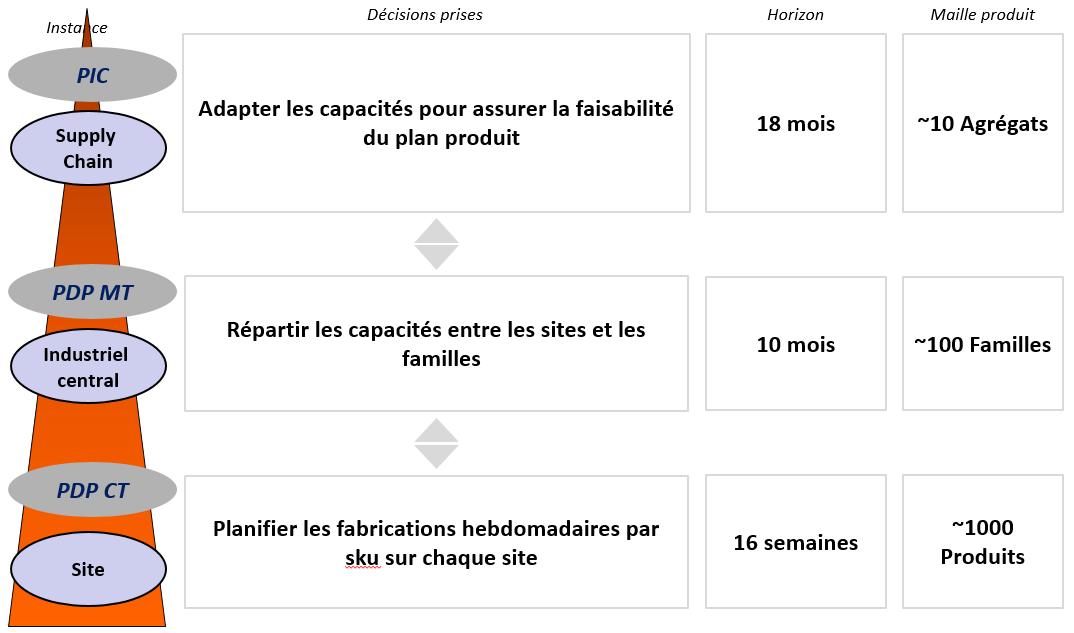
\includegraphics[width=\textwidth]{main/introduction/images/exemple_SC_luxe.png}
%   \caption{Exemple d'organisation de la Supply Chain d'un acteur du luxe}
%   \label{fig:exemple-SC-luxe}
% \end{figure}


% \section{Conséquences et problèmes étudiés}


% Optimsation multi-objectif : triangle coût / stock / service. (coût = coût hors stock).


% 2 sujets traités:
% \begin{itemize}
%   \item le niveau de multi-sourcing (moyen terme).
%   \begin{itemize}
%     \item Objectif : minimiser les coût de la création du multi-sourcing
%     \item Contrainte : taux de service client
%     \item Décisions : affectation produits / site
%   \end{itemize}
%   \item la plannification sous contrainte de flexibilité (court terme) décliné en deux axes :
%   \begin{itemize}
%     \item Optimization des paramètres des outils de PDP
%     \begin{itemize}
%       \item Objectif : minimiser le coût du stock
%       \item Contrainte : flexibilité industrielle (nombre de changements)
%       \item Décisions : Couverture de la production de chaque produits
%     \end{itemize}
%     \item Création du PDP en intégrant directement la contrainte de flexibilité
%     \begin{itemize}
%       \item Objectif : minimiser le coût du stock
%       \item Contrainte : flexibilité industrielle (nombre de changements)
%       \item Décisions : période de production et quantité produite pour chaque produit
%     \end{itemize}
%   \end{itemize}
% \end{itemize}


% Parler de la flexibilité du mix produit ! C'est ce qu'on optimise (ie : volume constant.)